
\tikzset{statenode/.style={circle, draw, very thick, minimum size=20mm}}
\tikzset{observnode/.style={rectangle, draw, very thick, minimum size=20mm}}
%\tikzset{loop/.style={looseness=10}}
\begin{figure}
	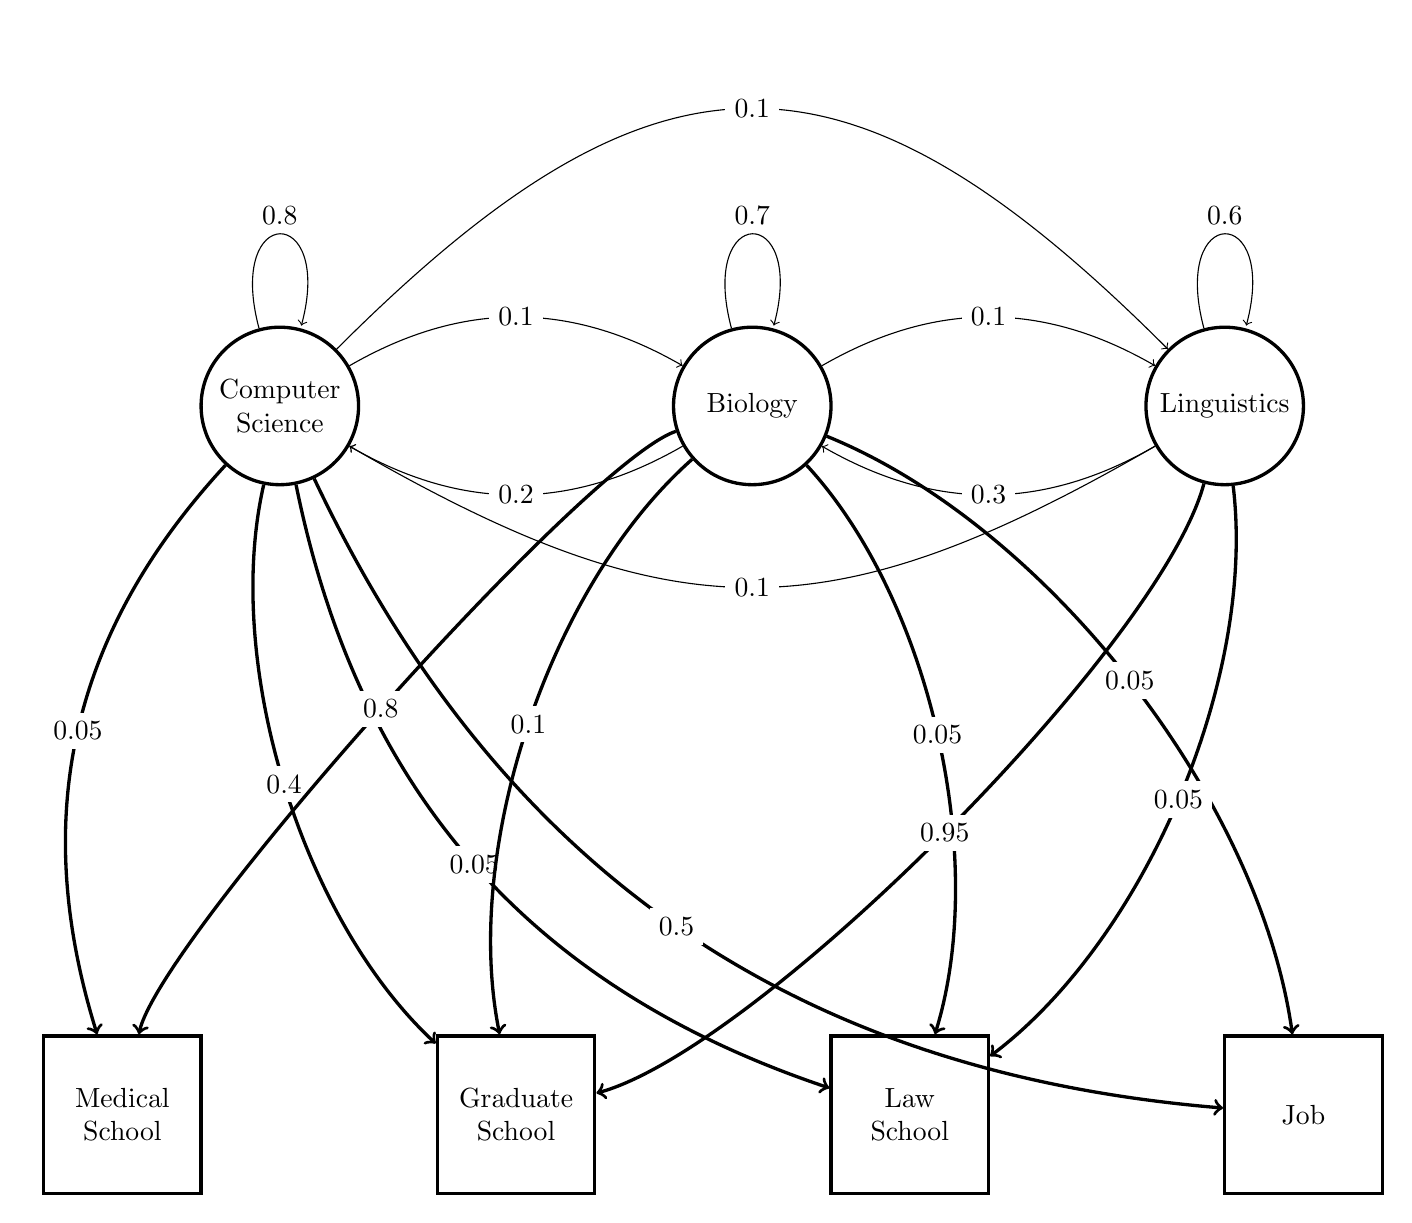
\begin{tikzpicture}
		%states
		\node[statenode] (CS) at (2,0) [draw, align=center] {Computer \\ Science};
		\node[statenode] (bio) at (8,0) {Biology};
		\node[statenode] (ling) at (14, 0) {Linguistics};


		%transition probabilities
		 \path[->] (CS) edge  [loop above] node {0.8} ();
		 \path[->] (CS) edge [bend left] node [fill=white] {0.1} (bio);
		 \path[->] (CS) edge [looseness = 1.4] node [fill=white] {0.1} (ling);

		 \path[->] (bio) edge [bend left] node [fill=white] {0.2} (CS);
		 \path[->] (bio) edge [loop above] node {0.7} ();
		 \path[->] (bio) edge [bend left] node [fill=white] {0.1} (ling);


		 \path[->] (ling) edge [bend left, looseness = 1.2] node [fill=white] {0.1} (CS);
		 \path[->] (ling) edge [bend left] node [fill=white] {0.3} (bio);
		 \path[->] (ling) edge [loop above] node {0.6} ();



		 %emission probabilities
		 \node[observnode] (med) at (0, -9) [draw, align=center] {Medical \\ School};
		 \node[observnode] (grad) at (5, -9) [draw, align=center] {Graduate \\ School};
		 \node[observnode] (law) at (10, -9) [draw, align=center] {Law \\ School};
		 \node[observnode] (job) at (15, -9) [draw, align=center] {Job};

		 \path[->, very thick] (CS) edge [bend right] node [fill=white] {0.05} (med);
		 \path[->, very thick] (CS) edge [bend right, looseness = 0.8] node [fill=white] {0.4} (grad);
		 \path[->, very thick] (CS) edge [bend right] node [fill=white, looseness = 0.6] {0.05} (law);
		 \path[->, very thick] (CS) edge [bend right] node [fill=white, looseness = 0.4] {0.5} (job);


		\path[->, very thick] (bio) edge [bend right, looseness = 0.3] node [fill=white] {0.8} (med);
		\path[->, very thick] (bio) edge [bend right, looseness = 0.8] node [fill=white] {0.1} (grad);
		\path[->, very thick] (bio) edge [bend left, looseness = 0.8] node [fill=white] {0.05} (law);
		\path[->, very thick] (bio) edge [bend left, looseness = 0.8] node [fill=white] {0.05} (job);



		\path[->, very thick] (ling) edge [bend left, looseness = 0.5] node [fill=white] {0.95} (grad);
		\path[->, very thick] (ling) edge [bend left, looseness = 0.8] node [fill=white] {0.05} (law);



	\end{tikzpicture}
	Figure 1. A Trellis diagram for the Hidden Markov Model example outlined in the introduction. Circles are possible states and squares are possible observations. Thin line represent state change probabilities and thick lines represent emission probabilities. 
\end{figure}